\documentclass{classrep}
\usepackage[utf8]{inputenc}
\frenchspacing

\usepackage{graphicx}
\usepackage[usenames,dvipsnames]{color}
\usepackage[hidelinks]{hyperref}
\usepackage{lmodern}
\usepackage{placeins}
\usepackage{url}
\usepackage{amsmath, amssymb, mathtools}
\usepackage{listings}
\usepackage{fancyhdr, lastpage}

\pagestyle{fancyplain}
\fancyhf{}
\renewcommand{\headrulewidth}{0pt}
\cfoot{\thepage\ / \pageref*{LastPage}}

%--------------------------------------------------------------------------------------%
\studycycle{Applied Information Technology, 2 cycle}
\coursesemester{II}

\coursename{Soft Computing Laboratory}
\courseyear{2021/2022}

\courseteacher{dr inż. Kamil Stokfiszewski}
\coursegroup{Wednesday, 8:30}

\author{%
    \studentinfo[239671@edu.p.lodz.pl]{Jan Karwowski}{239671}\\
    \studentinfo[239676@edu.p.lodz.pl]{Kamil Kowalewski}{239676}\\
}

\title{Assignment 3.: Multilayer Perceptron}

\begin{document}
    \maketitle
    \thispagestyle{fancyplain}

    \tableofcontents
    \newpage

    \section{Main goal}
    \label{main_goal} {
        The main goal of this task is to prepare implementation of multilayer perceptron and train
        it on simple pattern using backpropagation method. In scope of experiments hidden
        representation and impact of bias should be explored.
    }

    \section{Theoretical background} \label{theory} {
        Multilayer perceptron is a classic artificial neural network architecture, which consists of
        layers of neurons. Each layer contains neurons and share inputs between all these basic
        units. All outputs values from layer $n$ are provided as input values to layer $n+1$.
        Architecture used in this task is presented on fig. \ref{fig:multilayer_perceptron}.
        \begin{figure}[!htbp]
            \centering
            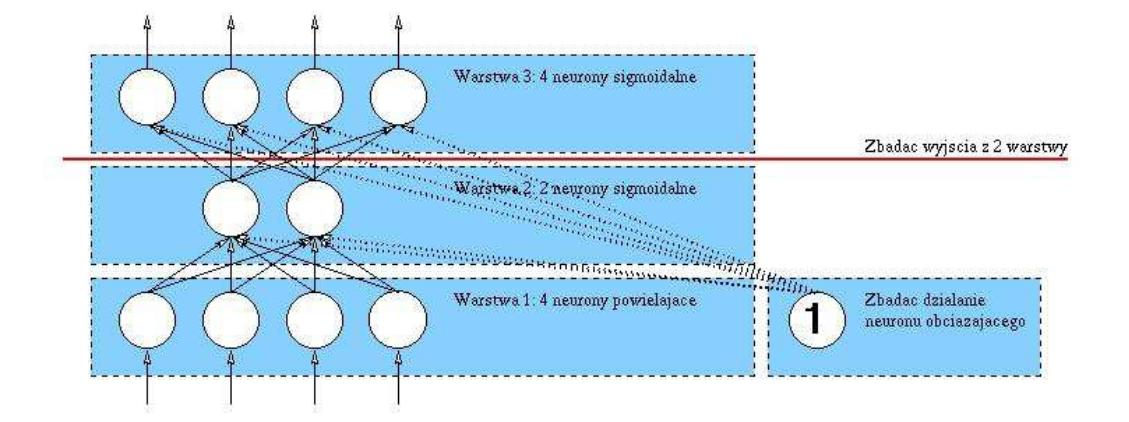
\includegraphics[width=0.9\textwidth]{img/multilayer_perceptron.jpg}
            \caption{Multilayer perceptron architecture}
            \label{fig:multilayer_perceptron}
        \end{figure}
        \FloatBarrier

        Layer output values could be processed by activation function, e.g. sigmoidal function:
        \begin{equation}
            f(x) = \frac{1}{1 - e^{-x}}
        \end{equation}
        Example input patterns used to train such a network:
        \begin{enumerate}
            \item 1.0 0.0 0.0 0.0 \verb|->| 1.0 0.0 0.0 0.0
            \item 0.0 1.0 0.0 0.0 \verb|->| 0.0 1.0 0.0 0.0
            \item 0.0 0.0 1.0 0.0 \verb|->| 0.0 0.0 1.0 0.0
            \item 0.0 0.0 0.0 1.0 \verb|->| 0.0 0.0 0.0 1.0
        \end{enumerate}
        As you can see, this is just an identity function on four input variables.
    }

    \section{Implementation} \label{implementation} {
        We implemented multilayer perceptron and backpropagation algorithm in C language, without
        support of any dedicated math or deep learning library. Only basic mathematical operation
        was used. The final program is build from two independent modules. The first one, called
        ,,autograd'' is our own implementation of automatic differentiation algorithm (i.e.
        general backpropagation algorithm). Details of this algorithm are described below. The
        second module contains implementation of multilayer perceptron, which uses ,,autograd''
        module to compute gradients of layers' weights. In this second module, structure and forward
        operation of MLP is defined. Also training loop, input/output operations, and testing
        process was implemented in scope of that. Whole logic contained in the second module follows
        classic ideas and is simple to understand, so it won't be explained in details.

        \subsection{Automatic differentiation} {
            ,,Autograd'' module is created to provide general algorithm to calculate derivatives of
            selected variables in ,,almost'' any function. In this case, function stands for some
            mathematical operation which has at least single input and exactly one output. Generally
            speaking this method is based on chain rule, i.e. it is based on calculation derivative
            of composite function.

            To find derivatives (gradient) of some function, this function has to be defined.
            Especially, it has to be defined as composite of some ,,basic'' functions. The set of
            these ,,basic'' functions (e.g. addition, multiplication or logarithm) is predefined
            in the module (or in the library in general). Assuming, that we have some composite
            function, consisting of some basic functions, which derivatives are known for, we are
            able to easily calculate derivative of the composite function using mentioned above
            ,,chain rule''. This process is presented in fig. \ref{fig:autograd}.

            \begin{figure}[!htbp]
                \centering
                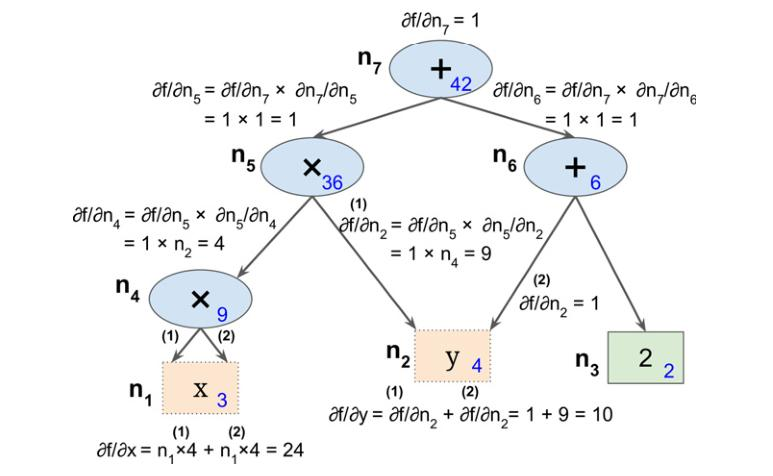
\includegraphics[width=0.9\textwidth]{img/autograd.jpg}
                \caption{Automatic differentiation method based on chain rule}
                \label{fig:autograd}
            \end{figure}
            \FloatBarrier

            Both definitions of basic functions and their derivatives are predefined in the source
            code of ,,autograd'' module. There is also defined a basic type ,,Double'', which is the
            core of the module and stores the history of operations, which is the result of. I.e
            this object is a node in the operations graph, and when some calculations are processed
            this graph is extended. When calculations are finished, then ,,backpropagation'' method
            can be executed and graph is explored from the last operation result (root) to all the
            variables (leaves) and basing on the chain rule derivatives of these variables are
            calculated.

            The last thing to clarify is a connection between this module, with its ability to
            calculate gradient of arbitrary function, and the artificial neural network. It's pretty
            simple, when we consider neural network as not so much complicate composition (a graph)
            of basic functions, which are addition, multiplication and sigmoid in the case of
            applied architecture of multilayer perceptron. In the MLP module, all the layers was
            defined using operations from this module, and this makes it simple, to find derivatives
            of mean squared error loss function after layers' weights.
        }
    }

    \section{Experiments and results} \label{results} {
        To study hidden representation of input (outputs from hidden layer) and examine bias impact on
        multilayer perceptron training ability, four experiments were conducted. All
        these attempts share common following parameters:
        \begin{itemize}
            \item number of layers and number of neurons in layers (fig. \ref{fig:multilayer_perceptron})
            \item neurons activation function (sigmoidal)
            \item number of training epochs - $100 000$
            \item learning rate - $0.1$
            \item input patterns as described in chapter \ref{theory}
        \end{itemize}
        Experiments differ in BIAS neuron presence, which is described by following scheme:
        \begin{enumerate}
            \item no bias
            \item bias in hidden and output layers
            \item bias in hidden layer only
            \item bias in output layer only
        \end{enumerate}
        where index of the list stands for experiment's number.  Results of these four experiments
        are presented in tables \ref{tab:with_bias_results}, \ref{tab:without_bias_results},
        \ref{tab:0with_bias_results} and \ref{tab:1with_bias_results}.

        \begin{table}[!htbp]
            \centering
            \begin{tabular}{|c|c|c|}
                \hline
                input values & hidden layer outputs & MLP outputs \\ \hline
                1.0 0.0 0.0 0.0 & 0.0000 0.0052 & 0.9893 0.0063 0.0107 0.0000 \\
                0.0 1.0 0.0 0.0 & 0.4805 1.0000 & 0.0060 0.9870 0.0000 0.0380 \\
                0.0 0.0 1.0 0.0 & 0.9398 0.0749 & 0.0058 0.0000 0.9828 0.0472 \\
                0.0 0.0 0.0 1.0 & 0.9379 0.5571 & 0.0006 0.0124 0.0150 0.9433 \\ \hline
            \end{tabular}
            \caption{Results of trained MLP WITH bias in hidden and output layers}
            \label{tab:with_bias_results}
        \end{table}
        \FloatBarrier

        \begin{table}[!htbp]
            \centering
            \begin{tabular}{|c|c|c|}
                \hline
                input values & hidden layer outputs & MLP outputs \\ \hline
                1.0 0.0 0.0 0.0 & 0.0000 0.0000 & 0.5000 0.5000 0.5000 0.5000 \\
                0.0 1.0 0.0 0.0 & 0.9999 0.0002 & 0.0046 0.9929 0.0000 0.2831 \\
                0.0 0.0 1.0 0.0 & 0.1790 0.9997 & 0.0074 0.0004 0.9691 0.5523 \\
                0.0 0.0 0.0 1.0 & 0.5995 0.9991 & 0.0008 0.0031 0.0321 0.4549 \\ \hline
            \end{tabular}
            \caption{Results of trained MLP WITHOUT bias in hidden and output layers}
            \label{tab:without_bias_results}
        \end{table}
        \FloatBarrier

        \begin{table}[!htbp]
            \centering
            \begin{tabular}{|c|c|c|}
                \hline
                input values & hidden layer outputs & MLP outputs \\ \hline
                1.0 0.0 0.0 0.0 & 0.0000 0.0000 & 0.5000 0.5000 0.5000 0.5000 \\
                0.0 1.0 0.0 0.0 & 0.9894 0.0002 & 0.0048 0.9922 0.0000 0.2899 \\
                0.0 0.0 1.0 0.0 & 0.2067 0.9999 & 0.0063 0.0006 0.9731 0.5526 \\
                0.0 0.0 0.0 1.0 & 0.6381 0.9995 & 0.0006 0.0049 0.0280 0.4552 \\ \hline
            \end{tabular}
            \caption{Results of trained MLP with bias in HIDDEN LAYER ONLY}
            \label{tab:0with_bias_results}
        \end{table}
        \FloatBarrier

        \begin{table}[!htbp]
            \centering
            \begin{tabular}{|c|c|c|}
                \hline
                input values & hidden layer outputs & MLP outputs \\ \hline
                1.0 0.0 0.0 0.0 & 0.0000 0.0000 & 0.9895 0.0022 0.0090 0.0000 \\
                0.0 1.0 0.0 0.0 & 0.5410 1.0000 & 0.0062 0.9870 0.0000 0.0430 \\
                0.0 0.0 1.0 0.0 & 0.9998 0.0001 & 0.0052 0.0000 0.9866 0.0511 \\
                0.0 0.0 0.0 1.0 & 0.9998 0.5198 & 0.0006 0.0130 0.0116 0.9370 \\ \hline
            \end{tabular}
            \caption{Results of trained MLP with bias in OUTPUT LAYER ONLY}
            \label{tab:1with_bias_results}
        \end{table}
        \FloatBarrier
    }

    \section{Summary and conclusions} \label{summary} {
        Basing on results presented in the tables we can observe that bias is required to train MLP
        on this particular pattern. We can see that MLP outputs are almost same as input values in
        tables \ref{tab:with_bias_results} and \ref{tab:1with_bias_results}. So during these two
        experiments network was successfully trained. On the other hand in tables
        \ref{tab:without_bias_results} and \ref{tab:0with_bias_results} presents unsuccessful
        trainings, where MLP output values are correct only for the part of the input patterns - for
        pattern two and three. Basin on these two observations we can draw a conclusion that BIAS
        neuron in output layer is a key component, required to train network successfully.

        Given the above conclusion we should consider hidden layer output values to understand, why
        this BIAS neuron is required to train the multilayer perceptron. Hidden layer output values
        are a kind of encoded inputs - input patterns consisting of 4 scalar values  are presented
        using only 2 scalar values. These hidden representation method should be so clever to
        produce different representation for each input pattern, to finally let output neurons
        differentiate between all the four kind of inputs. Successful training results present
        hidden representations, which in fact are different for each input pattern. We can observe
        both hidden inputs set to min value (0.0), single high value, and two pairs of high and mid
        values.  So this is relatively simple to produce four different hidden representation for
        these four input patterns. Let's say, this is especially simple for the human, to find and
        differentiate between these representations. But the problem appears when it comes to output
        neurons. These units have to be able to differentiate between hidden representations using
        two weights, single addition or subtraction operation and optional offset value(BIAS
        neuron). As we can see in our experiments, this offset value is a key component of neuron
        operation, which lets him to differentiate between above hidden representation. For example,
        it can not fully activate when both hidden layer output values are set to 0.0 without
        offset. In fact, since this particular training method we used (backpropagation), proper
        hidden representation have been not even found for models without BIAS in output layer. So
        the final conclusion is: BIAS neuron in output layer is required to learn these four input
        patterns because of ability to found and understand hidden representation, which consists of
        two values only.
    }

    \begin{thebibliography}{0}
        % @formatter:off
        \bibitem{instruction}{Labolatory instruction, URL: https://ftims.edu.p.lodz.pl/pluginfile.php/75440/\\mod\_resource/content/1/soft\_comp\_lab\_03\_PERCEPTRON.pdf}
        % @formatter:on
    \end{thebibliography}

\end{document}
